% ========== RÆV ==========
\begin{frame}{%
  \begin{minipage}[c]{0.30\textwidth}
    Ræv
  \end{minipage}%
  \hfill
  \begin{minipage}[c]{0.45\textwidth}
    \footnotesize
    \textbf{Jagttid:} 1.\ september -- 31.\ januar
  \end{minipage}%
  \hfill
  \begin{minipage}[c]{0.15\textwidth}
    \noindent\raggedleft
    
\includegraphics[width=0.5cm, height=0.5cm, keepaspectratio]{Billeder/Ikoner/star.png}%
    \hspace{0.2em}%
    
\includegraphics[width=0.5cm, height=0.5cm, keepaspectratio]{Billeder/Ikoner/star.png}%
    \hspace{0.2em}%
    
\includegraphics[width=0.5cm, height=0.5cm, keepaspectratio]{Billeder/Ikoner/star.png}
  \end{minipage}%
}
  \vspace{0.25em}
  \begin{columns}[T]
    % --- Venstre kolonne: Tekst ---
    \column{0.45\textwidth}
    \setlength{\parskip}{0.4em}
    \tiny
    \RaggedRight
    \textbf{\textit{Vulpes vulpes}} – udbredt hundedyr, der er ekstremt tilpasningsdygtigt og ses overalt i Danmark. \par
    \textbf{Udseende:}\\
    \quad – Overvejende rød \\
    \quad – Hvid bug \\
    \quad – Markant rød hale \\
    \quad – Sorte aftegninger \par
    \textbf{Levesteder:} Alle landskabstyper. \par
    \textbf{Føde:} Smågnavere, fugle, bær, biller, ådsler, harekillinger og rålam. \par
    \textbf{Sygdomme:} Ræveskab, rævens dværgbændelorm, hvalpesyge. \par
    \textbf{Parring:} Sidst i januar / start februar (rolletiden). \par
    \textbf{Forplantning:}\\
    \quad – \textbf{Kønsmoden:} 1 år \\
    \quad – \textbf{Mono/polygam:} Monogam \\
    \quad – \textbf{Bestandsomsætning:} Middel \\
    \quad – \textbf{Kuld:} 4--7 hvalpe
    % --- Højre kolonne: Større billede ---
    \column{0.52\textwidth}
    \centering
    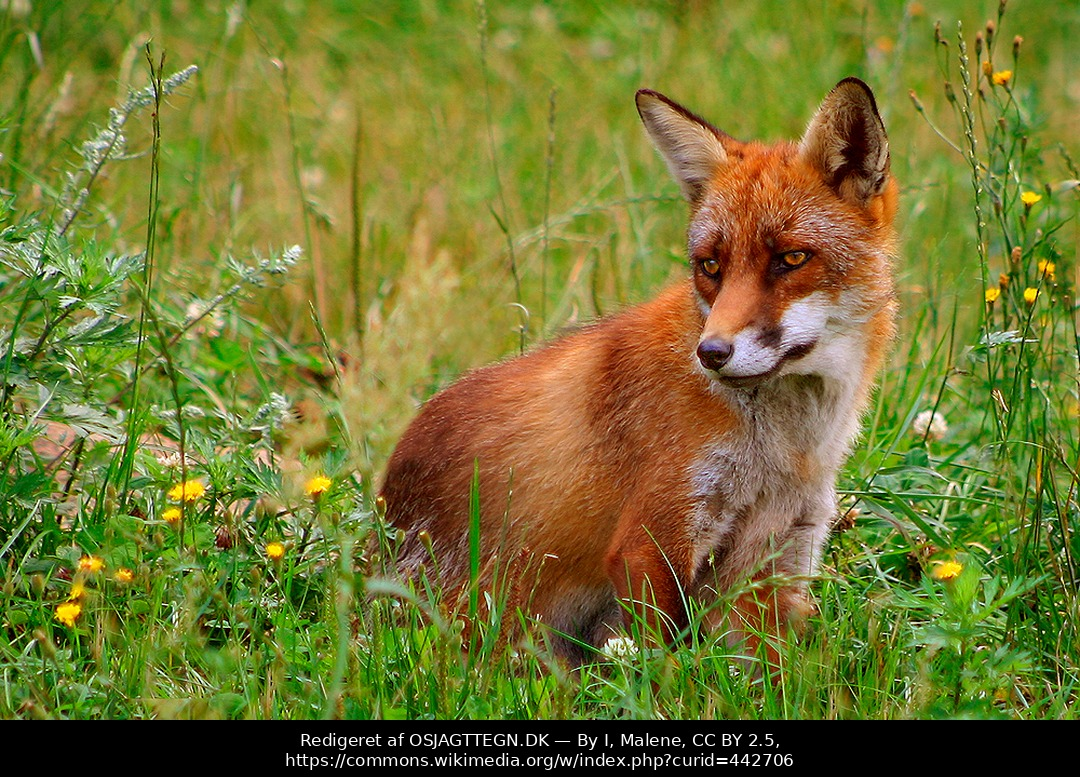
\includegraphics[width=\linewidth, height=7.2cm, keepaspectratio]{Billeder/Dyr/Pattedyr/rovdyr/ræv/raev-10.jpg}
  \end{columns}
\end{frame}